% http://www.ctan.org/tex-archive/macros/latex/contrib/beamer/examples
% http://latex.artikel-namsu.de/english/beamer-examples.html

%\documentclass{beamer}
\documentclass[usenames,dvipsnames]{beamer}
\usepackage{amsmath}
\usepackage{amssymb}
\usepackage{bm}
\usepackage{fancybox, graphicx}
\usepackage{listings}
\usepackage{tikz} % Diagrams
\usepackage{color}
\usepackage{textcomp} % See https://tex.stackexchange.com/questions/145416/how-to-have-straight-single-quotes-in-lstlistings

\lstset{language=bash,upquote=true} % Format listings as appropriate for bash. Inexplicably we get problems if the language is set as part of the \begin{lstlisting} command.

% https://tex.stackexchange.com/questions/36030/how-to-make-a-single-word-look-as-some-code
\definecolor{light-gray}{gray}{0.95}
\newcommand{\code}[1]{\colorbox{light-gray}{\texttt{#1}}}



\usetheme{boxes}
\usecolortheme{beaver}


\title{Introduction to Computing with GPUs}
\author{Lorne Whiteway \\ lorne.whiteway@star.ucl.ac.uk}
\institute{Astrophysics Group \\ Department of Physics and Astronomy \\ University College London}
\date{August 2018}

\subject{IT}

\begin{document}

\frame{\titlepage}


\begin{frame}{Where to find this presentation}
  \begin{block}{}
    Find the presentation at \alert{\url{https://tinyurl.com/XXXXXXX}}.\\
  \end{block}
  \begin{block}{}
    On this page click on `Download' to get a copy of the presentation.
  \end{block}
\end{frame}

\begin{frame}{Motivation}
  \begin{block}{}
    \begin{itemize}
      \item{This presentation summarises material from the (excellent) course `CUDA Programming on NVIDIA GPUs' by Mike Giles, Oxford.}\\~\
      \item{\url{http://people.maths.ox.ac.uk/~gilesm/cuda/}}
    \end{itemize}
  \end{block}
\end{frame}

\begin{frame}{Two paradigms}
  \begin{block}{}
    \begin{itemize}
      \item{Intel (market cap \$220B\footnotemark): One-chip-fits-all. Use the same chip (a CPU) for all tasks (e.g. both word processing and high-performance computing (HPC)).}\\~\
      \item{NVIDIA (market cap \$152B\footnotemark[\value{footnote}]): Create a specialised chip (the GPU) specifically tailored for certain tasks (including HPC).}
    \end{itemize}
  \end{block}
  \footnotetext[\value{footnote}]{As of 27 July 2018}
\end{frame}

\begin{frame}{GPUs}
  \begin{block}{}
    \begin{itemize}
      \item{GPU  = graphics processing unit}
      \item{Specialised chip}
      \item{Has many processors and a specialised memory structure}
      \item{Designed specifically for high performance via parallelisation when doing graphics rendering.}
      \item{Single instruction, multiple data (SIMD).}
      \item{This design also makes them suitable for parallelizable problems in HPC.}
      \item{Not-standalone - need a CPU `host'.}
    \end{itemize}
  \end{block}
\end{frame}

\begin{frame}{GPUs are displacing CPUs for HPC}
  \begin{block}{}
    \begin{itemize}
      \item{GPUs offer better value (FLOPS/\$) and energy usage (FLOPS/J) than CPUs.}\\~\
      \item{5 of the world's top 7 supercomputers use GPUs.\footnotemark}\\~\
      \item{All else being equal, we should probably use GPUs for HPC...}
    \end{itemize}
  \end{block}
\footnotetext[\value{footnote}]{As of June 2018}
\end{frame}

\begin{frame}{But...}
  \begin{block}{}
    \begin{itemize}
      \item{Installed base of CPUs (e.g. splinter).}\\~\
      \item{Takes time to develop GPU expertise.}\\~\
      \item{Program code needs to be altered to run (effectively) on GPUs.}
    \end{itemize}
  \end{block}
\end{frame}

\begin{frame}{GPUs on splinter}
  \begin{block}{}
    \begin{itemize}
      \item{New (July 2018) GPU `Tesla V100' (in addition to old `K80').}\\~\
      \item{Thanks to Ofer (funding) and Edd (implementation)!}\\~\
      \item{How can we use these cards effectively?}
    \end{itemize}
  \end{block}
\end{frame}

\begin{frame}{Tesla V100 specifications} {\tiny \url{http://www.nvidia.com/content/PDF/Volta-Datasheet.pdf}}
  \begin{block}{}
    \begin{center}
      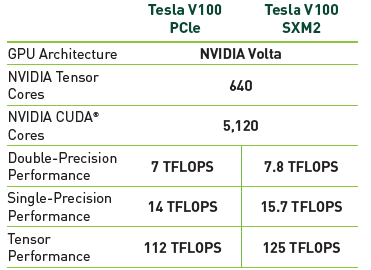
\includegraphics[scale=0.90]{V100_specsheet_A.png}
    \end{center}
  \end{block}
\end{frame}

\begin{frame}{Tesla V100 specifications} {\tiny \url{http://www.nvidia.com/content/PDF/Volta-Datasheet.pdf}}
  \begin{block}{}
    \begin{center}
      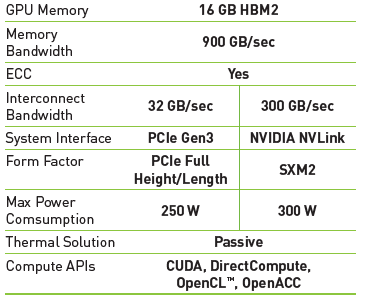
\includegraphics[scale=0.83]{V100_specsheet_B.png}
    \end{center}
  \end{block}
\end{frame}

\begin{frame}{Next problem...}
  \begin{block}{}
    \begin{itemize}
      \item{When you solve your biggest problem you simply get a new biggest problem.}\\~\
      \item{Large number of processors should slash computation wallclock time for parallelizable problems.}\\~\
      \item{But in fact we simply discover that speed of memory read/write becomes the new bottleneck.}\\~\
    \end{itemize}
  \end{block}
\end{frame}

\begin{frame}{GPU memory hierarchy}
  \begin{block}{}
    \begin{itemize}
      \item{Use a \textit{memory hierarchy} (moving down the list: faster, smaller, more expensive):}
      \begin{itemize}
      \item{CPU (`host') core memory}
      \item{GPU (`device') core memory}
      \item{Level 2 (`L2') cache}
      \item{Level 1 (`L1') cache}
      \item{Registers}
      \end{itemize}
      \item{Data transfer links as fast as possible. But e.g. CPU host $\leftrightarrow$ GPU device is relatively slow.}\\~\
      \item{Not just a hardware issue - GPU-destined software must be written with memory access speed in mind as well.}\\~\
    \end{itemize}
  \end{block}
\end{frame}

\begin{frame}{CPU $\leftrightarrow$ GPU relatively slow}
  \begin{block}{}
    \begin{itemize}
      \item{Data transfer links as fast as possible. But e.g. CPU host $\leftrightarrow$ GPU device is relatively slow.}\\~\
      \item{Some problems are simply not worth doing on the GPU as it would be slower to copy the data to the GPU than it would be to do the calculation non-parallel on the CPU.}\\~\
      \item{Not worth copying a number to the GPU unless you are going to do roughly 100 FLOPS with it.}\\~\
      \item{But e.g. matrix multiplication is certainly worth doing on the GPU as copying data is $\mathcal{O}(N^2)$ while the calculation is $\mathcal{O}(N^3)$.}\\~\
    \end{itemize}
  \end{block}
\end{frame}

\begin{frame}{Parallel Programming - threads}
  \begin{block}{}
    \begin{itemize}
      \item{The code that runs on the GPU should create multiple threads; one thread will get attention from one processor.}\\~\
      \item{Generally you want many, many threads at the same time (to keep all the processors busy); if the problem is parallelizable then you should be able to orgamise the code to achieve this (e.g. each thread deals with part of the data).}\\~\
      \item{The threads will get batched into sets of 32 threads called `warps' and you want many such warps.}\\~\
    \end{itemize}
  \end{block}
\end{frame}

\begin{frame}{Parallel Programming - warps}
  \begin{block}{}
    \begin{itemize}
      \item{The 32 threads in a warp run in absolute lockstep - they all execute the same code at the same time on different data (SIMD).}\\~\
      \item{Consider \texttt{threadID < 8 ? f(x) : g(x);} here the first 8 threads calculate f while 24 threads twiddle their thumbs, \textbf{then} 24 threads calculate g while 8 threads twiddle their thumbs. Suboptimal.}\\~\
    \end{itemize}
  \end{block}
\end{frame}

\begin{frame}{GPU programming: CUDA}
  \begin{block}{}
    \begin{itemize}
      \item{CUDA is a language in which you can write code that will execute efficiently on a GPU.}\\~\
      \item{CUDA is \texttt{C}, plus templates, plus a few CUDA-specific language instructions. Use extention \texttt{.cu}.}\\~\
      \item{There is a CUDA compiler \texttt{nvcc} (I suspect that it's just a \texttt{C} preprocessor...)}\\~\
      \item{can link with other C, C++, Fortran object files.)}\\~\
    \end{itemize}
  \end{block}
\end{frame}

\begin{frame}{CUDA example - see handout}
  \begin{block}{}
    \begin{center}
      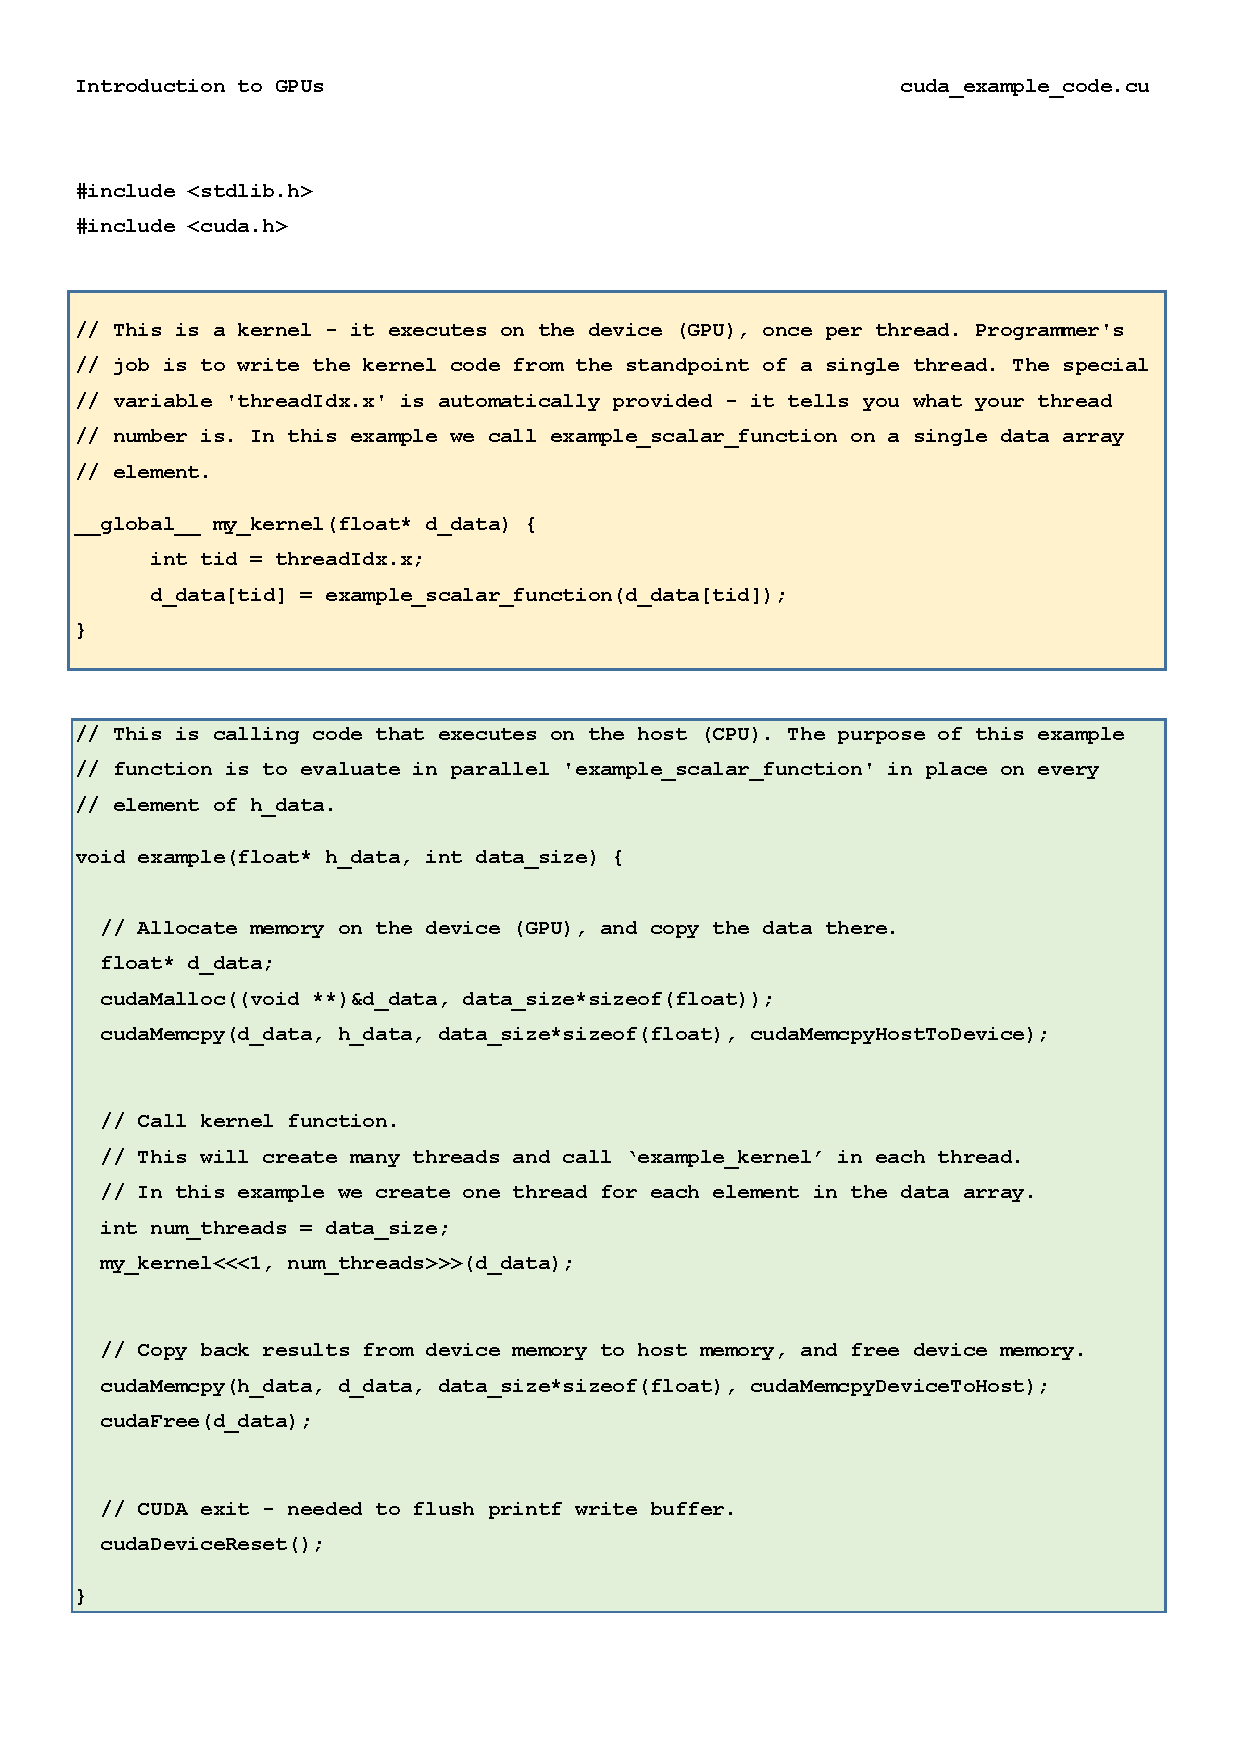
\includegraphics[scale=0.23]{cuda_example_code.pdf}
    \end{center}
  \end{block}
\end{frame}

\begin{frame}{CUDA example - host code (green)}
  \begin{block}{}
    \begin{itemize}
      \item{Need to copy data to device, so \texttt{malloc} then \texttt{memcpy}. But the host cannot see the device memory explicitly, so use special CUDA functions to do this.}\\~\
      \item{The `kernel' is the code that will run on the GPU. Special syntax $\langle\langle\langle \texttt{1, num\_threads} \rangle\rangle\rangle$ to specify number of threads; also has a normal argument list.}\\~\
    \end{itemize}
  \end{block}
\end{frame}

\begin{frame}{CUDA example - device code (yellow)}
  \begin{block}{}
    \begin{itemize}
      \item{Special keyword \texttt{\_\_global\_\_} identifies kernel function.}\\~\
      \item{Written from the point of view of one thread (like MPI, not like OpenMP).}\\~\
      \item{Special variable \texttt{threadIdx.x} automagically tells the kernel code what thread it is running in.}\\~\
    \end{itemize}
  \end{block}
\end{frame}

\begin{frame}{Organisation of threads}
  \begin{block}{}
    \begin{itemize}
      \item{32 threads in a warp - they move in absolute lockstep.}\\~\
      \item{Up to 32 warps in a \textit{block}. All the threads in a block can share some L1 cache memory.\footnotemark}\\~\
      \item{As many blocks as you want (running on one GPU). All threads in the GPU can share some L2 cache memory.}\\~\
      \item{There are also methods for running across multiple GPUs...}\\~\
    \end{itemize}
  \end{block}
\footnotetext{Maximum threads in a block depends on the GPU architecture}
\end{frame}

\begin{frame}{Organisation of threads}
  \begin{block}{}
    \begin{itemize}
      \item{Thus thread organisation is hierarchical (just as it was with memory organisation).}\\~\
      \item{This reflects a preference for `fine control at multiple levels' (in the persuit of maximum performance) at the cost of simplicity of design.}\\~\
    \end{itemize}
  \end{block}
\end{frame}

\begin{frame}{CUDA code with multiple thread blocks}
  \begin{block}{}
    \begin{itemize}
      \item{In the caller:\newline
      \texttt{int threads\_per\_block = 32;}\newline
      \texttt{int n\_blocks = data\_size / threads\_per\_block;}\newline
      \texttt{my\_kernel}$\langle\langle\langle$\texttt{n\_blocks, threads\_per\_block}$\rangle\rangle\rangle$\texttt{(d\_data);}
      }\\~\
      \item{In the kernel:\newline
      \texttt{int tid = threadIdx.x + blockDim.x * blockIdx.x}
      }
    \end{itemize}
  \end{block}
\end{frame}


\begin{frame}{Synchronisation}
  \begin{block}{}
    \begin{itemize}
      \item{Threads in a warp move in lockstep but otherwise no guarantees of synchronicity - thread 145 might finish before thread 13 begins.}
      \item{There are functions to implement syncorisation (across threads in a block, or across all blocks).}
      \item{Can set up some shared memory for all the threads in a block.}
      \item{There are some \textit{atomic} functions e.g. for modifying a global variable; your thread will briefly get a lock on the global variable.}
      \texttt{Very fast functions to allow threads in a warp to exchange information.}
    \end{itemize}
  \end{block}
\end{frame}

\begin{frame}{Cache lines}
  \begin{block}{}
    \begin{itemize}
      \item{Data is read in a \textit{cache line} of 64 bytes (8 doubles) - if you ask for only one double, you will still get 8. Only a few cache lines can be held in fast memory at a time.}
      \item{You will be used to this when programming CPUs. For example, it makes sense to process an array sequentially, so as not to `churn' the cache lines.}
      \item{Still an issue with GPUs, but here you need sensible interaction with the cache lines across \textit{all} the threads in a warp.}
    \end{itemize}
  \end{block}
\end{frame}


\end{document}
